\section{Component View}
In the figure below the high level component architecture of the System is presented. It is composed by two main modules that correspond to the two platforms used by the two different kinds of customers of our services: 
The \emph{Web application} is for the Third Parties, that use the System connecting to the site through a Web Browser, and interact with the \emph{Third Party Mobile Services} subsystem. The \emph{Mobile application} is for individual Users, which access the system with an iOS or Android device through the TrackMe Mobile Application, and interact with the \emph{User Mobile Service} subsystem.

\vspace{6mm}

\begin{figure}[H]

    \centering
    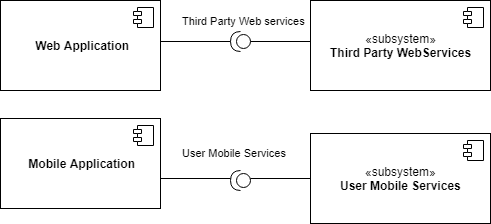
\includegraphics[scale=0.2]{./Pictures/component.png}
    \caption{Component view of \emph{TrackMe} system}
    
\end{figure}

\subsection{Component view of the Third Party Web Services}
\begin{figure}[H]

    \centering
    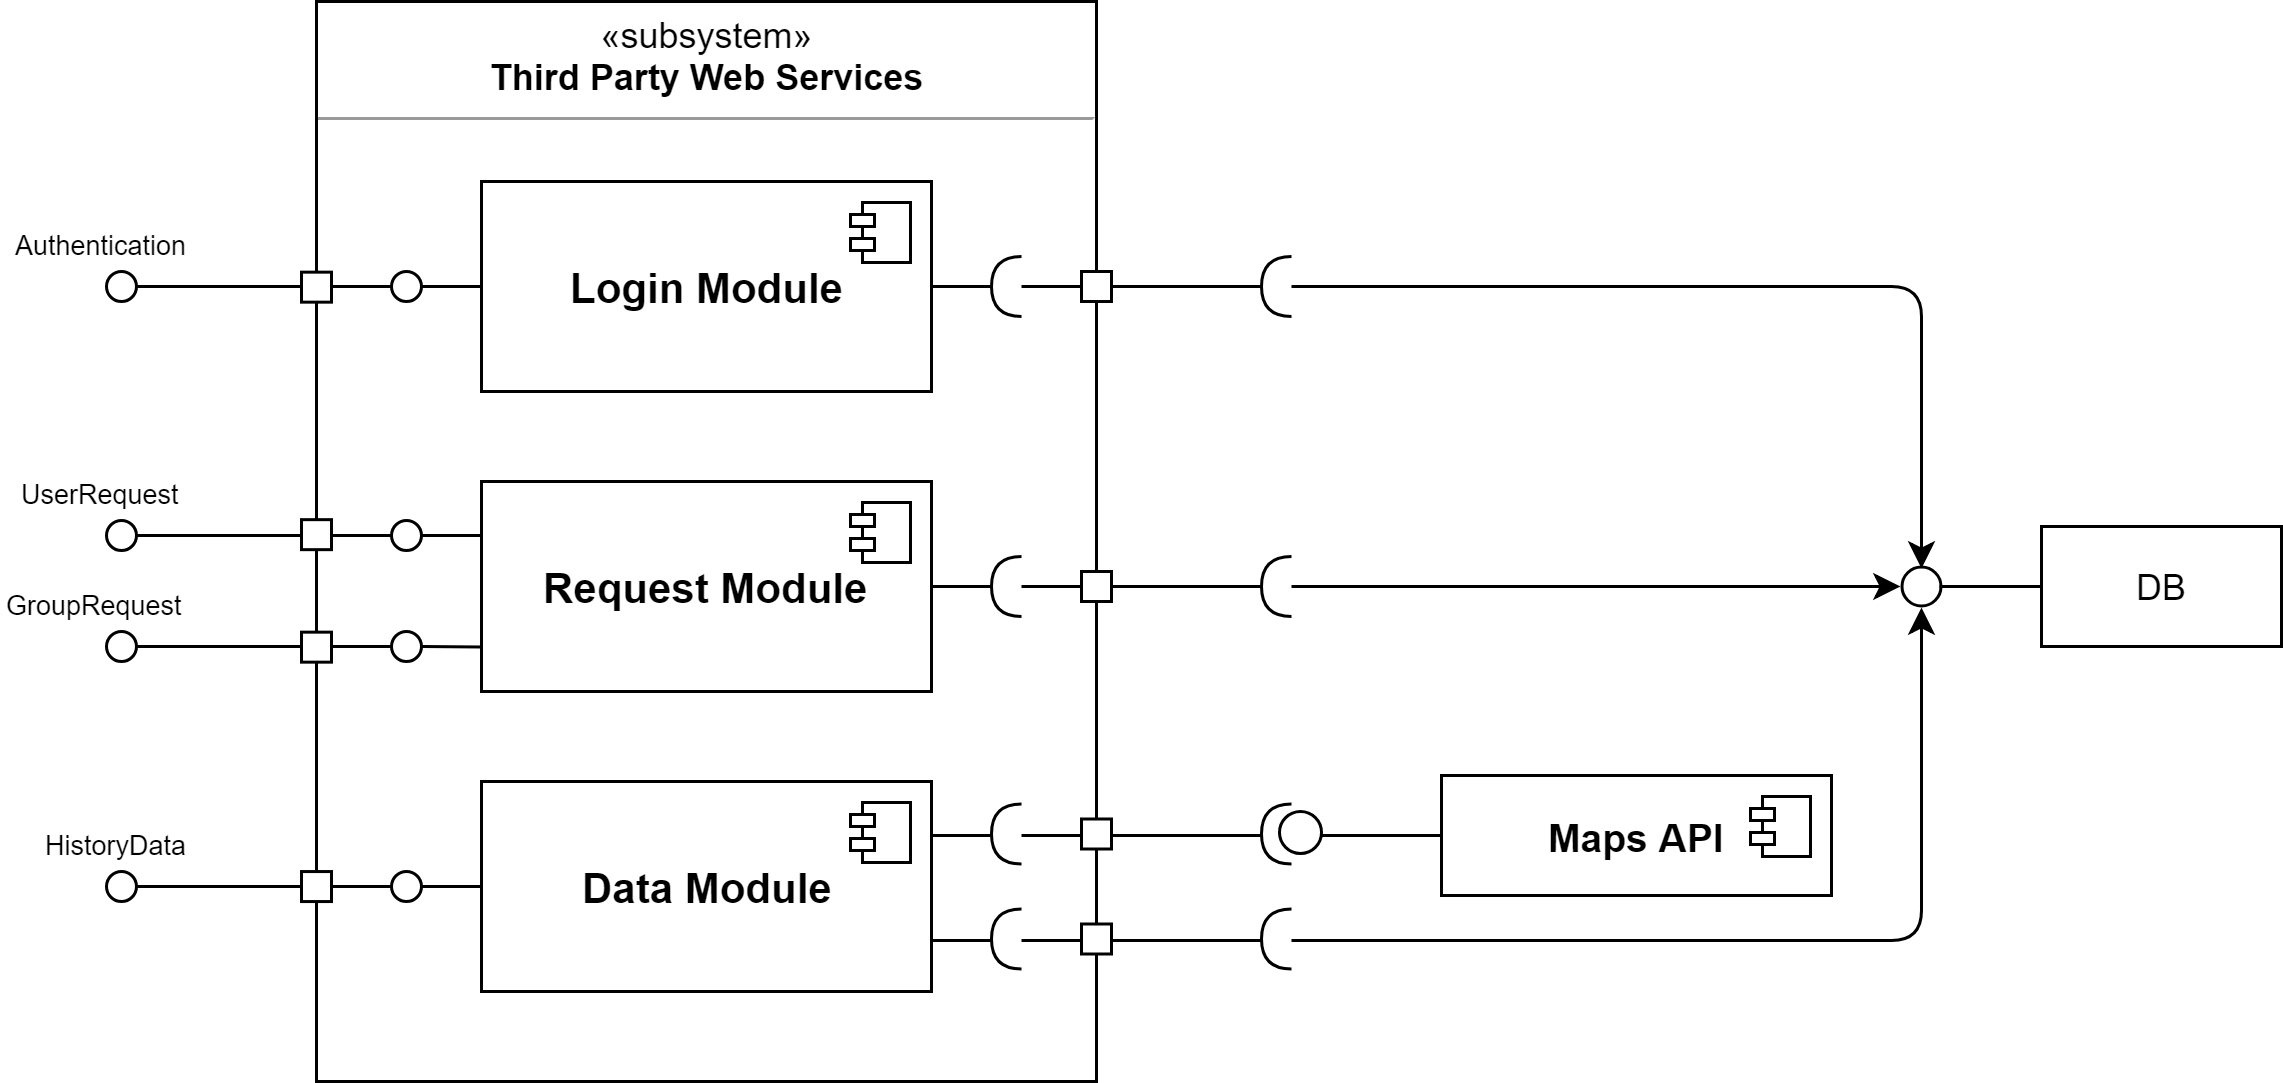
\includegraphics[scale=0.18]{./Pictures/thirdPartyServicesDiagram.png}
    \caption{Third Party Web Service component}
    
\end{figure}
    
\begin{itemize}
\item  The \emph{Login Module} manages the operations of authentication, allowing the Third Party to be recognized and to consequently use the services of the system. It interacts with the database to check the credentials and retrieve the account information.

\item The \emph{Request Module} is responsible for the requests dispatching: it offers to the Third Party the interfaces to fill out the forms to perform a user or a group request, and forward them to the database. Among its internal function, it sends a notification to the target User when he/she is the subject of a User Request and it performs the security check in case of  a Group Request, allowing it only if the group is composed of at least 1000 individuals.
    
\item The \emph{Data Module} offers to the Third Parties all the functionalities to manage the performed requests, grouped by status (pending, accepted and refused), allows the consultation of the results and calculates useful statistics on collected data. In case of subscription requests, it is its responsibility to update the Third Party with the new data available with the chosen frequency.
It retrieves data querying the database, where the User records are stored. In case of a Group Request, it also provides data anonymity.
This module is connected to the maps API to allow the consultation of a User's location data on an interactive map.
    
\end{itemize} 
   
\subsection{Component view of the User Mobile Service}

\begin{figure}[H]

    \centering
    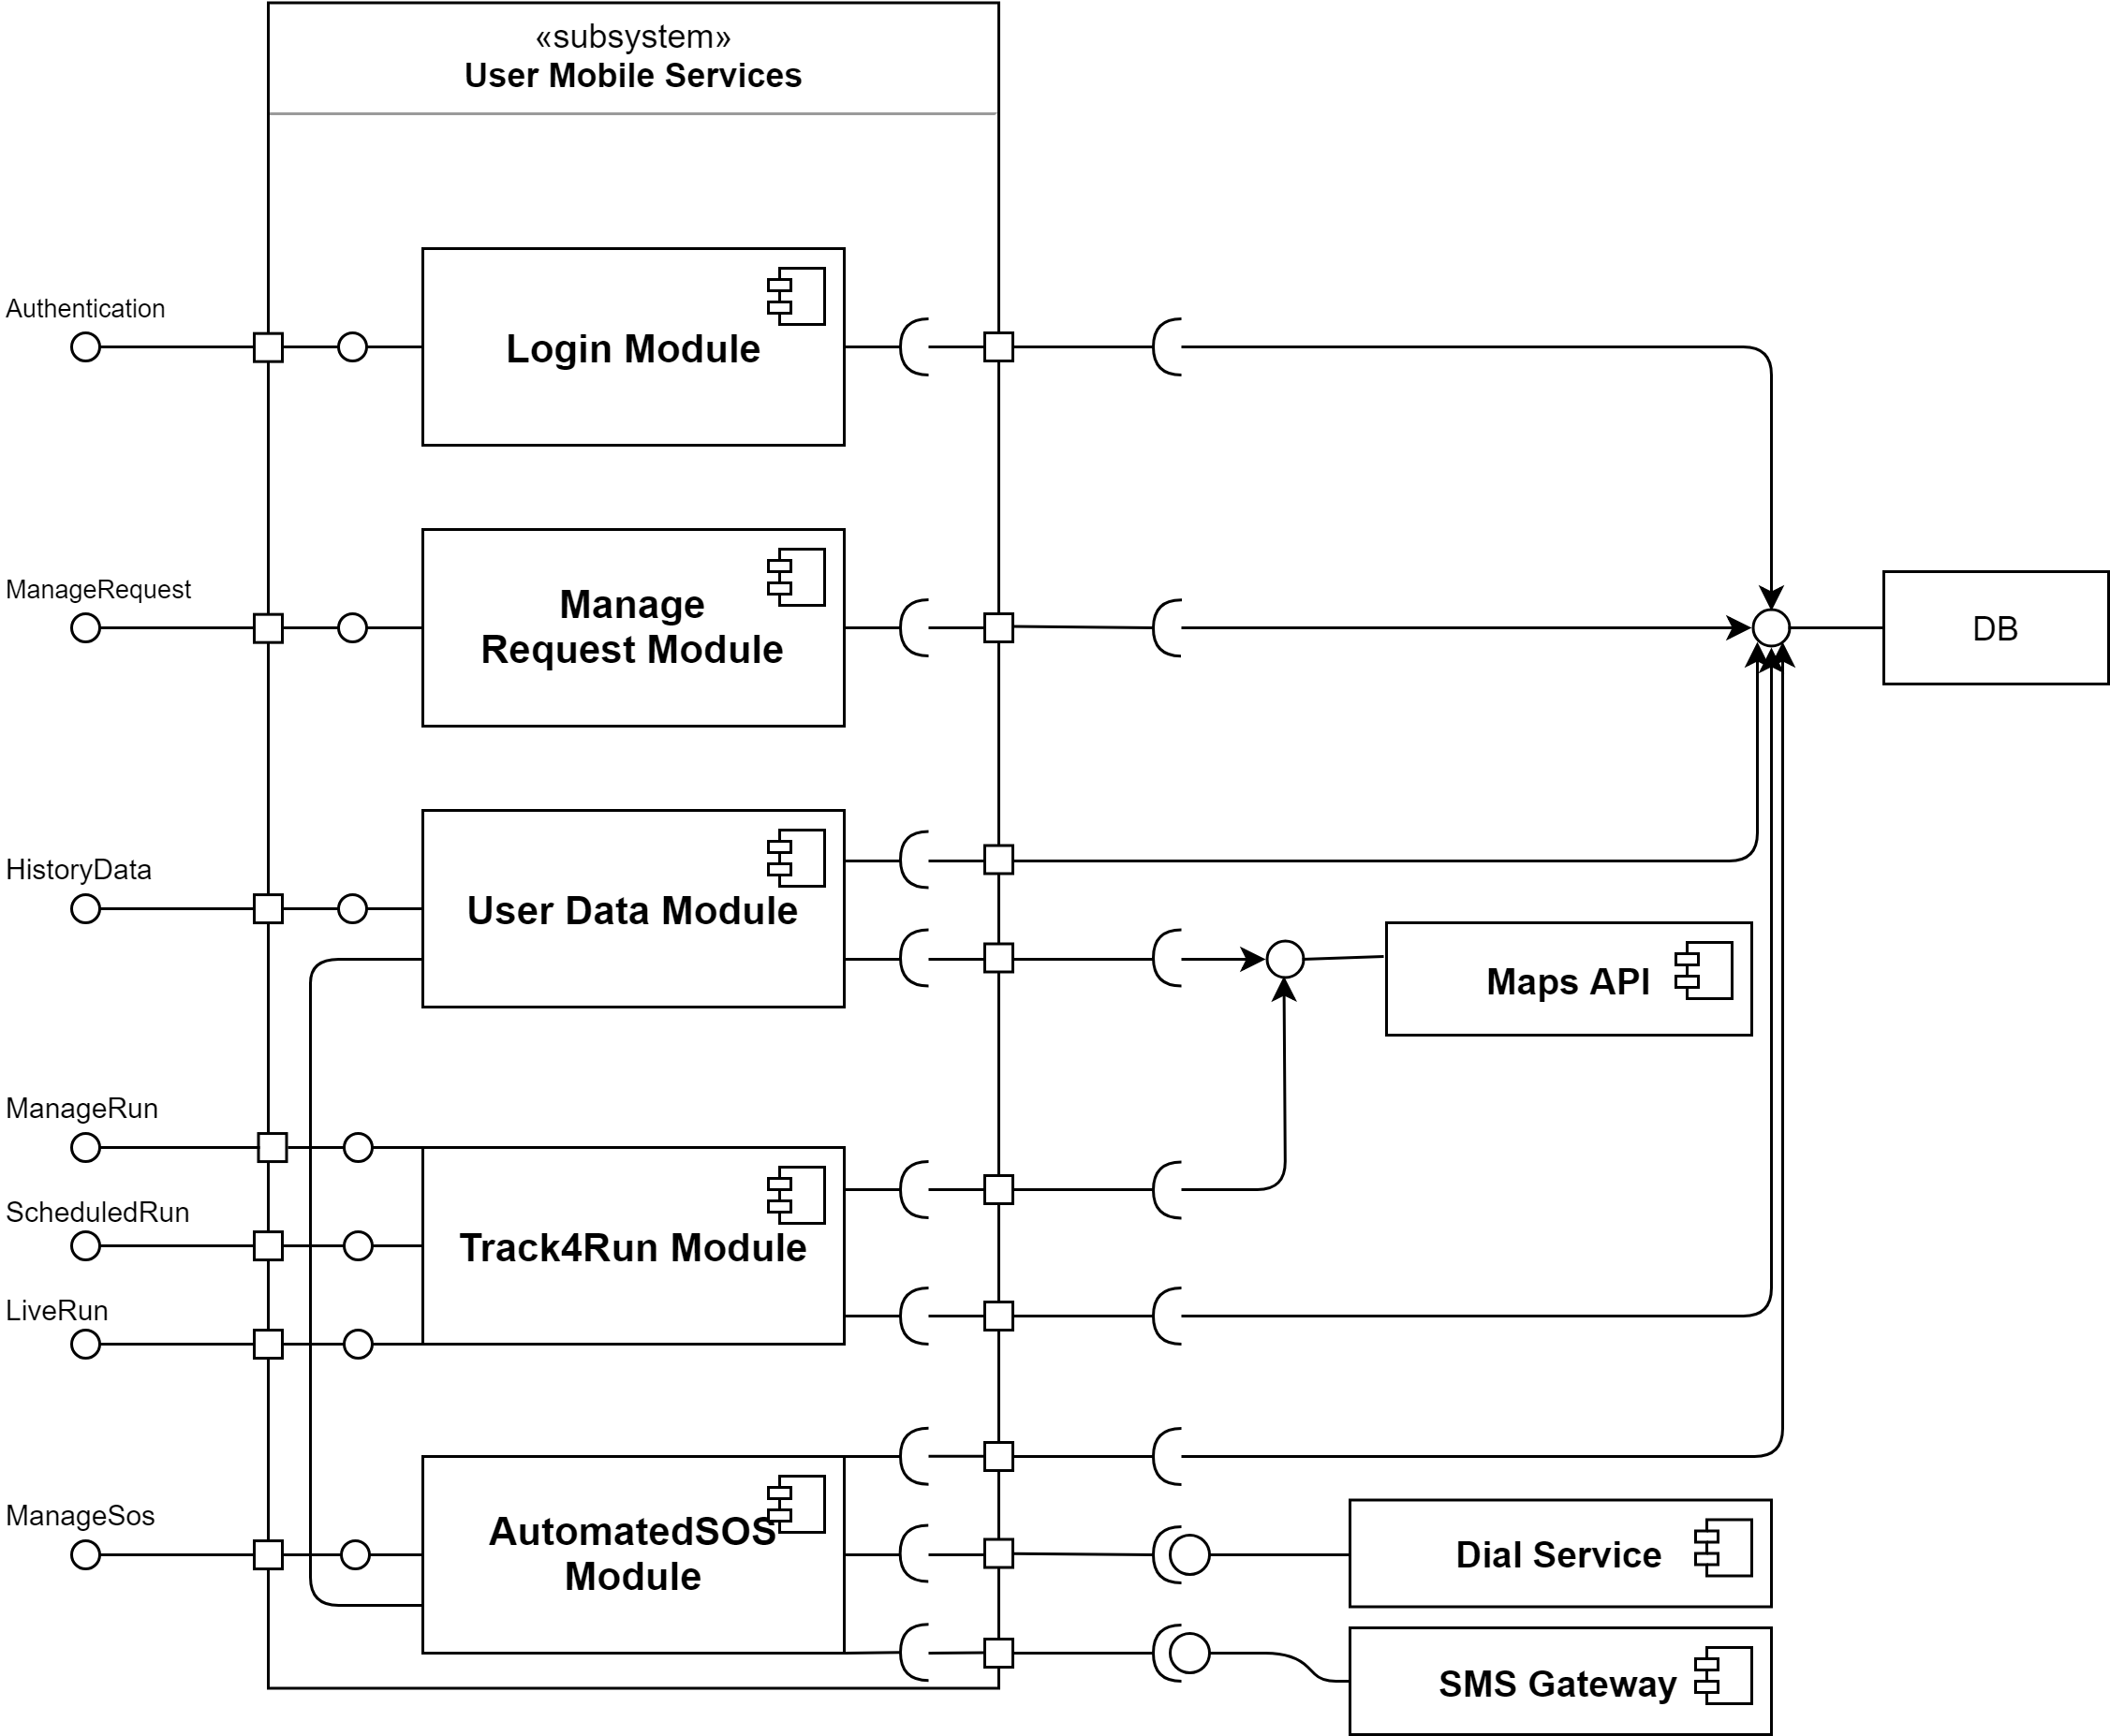
\includegraphics[scale=0.2]{./Pictures/userServicesDiagram.png}
    \caption{User Mobile Services component}
    
\end{figure}

\begin{itemize}
    \item The \underline{Login Module} manages the operations of authentication, allowing the User to be recognized and to use the services of the system. It interacts with the database to check the credentials and retrieve the account information.
    
    \item The \underline{Manage Request Module} offers to the User the functionalities to manage the incoming requests, providing all the information about the requested data. It interacts with the database, dispatches the User reply and notifies the sender Third Party about the occurred response.
    
    \item The \underline{User Data Module} sends the new User's health and location data to the database of the system, as soon as they have been collected by the smart device.
    It offers the interfaces that allow the User to visualize his/her History Data present in the database. It uses the maps API to allow the visualization of User location data on an interactive map.
    
    \item The \underline{Track4Run Module} works as Run manager for the Track4Run system: it offers to the User the interfaces that allow to create a run and enroll to it, to visualize the list of the planned runs and to follow live runs. It interacts with the maps API module, in order to manage the location data, and with the database, in order to store new runs and retrieve all the details about them.
    
    \item The \underline{AutomatedSOS module} provides the functionalities that concern the AutomatedSOS service: it offers to the User the interfaces that allow him/her to enable or disable the service, to manage the emergency contacts list and the emergency text message.
    It deals with all the tasks related to the emergency: it performs the checks on the health status and notifies an emergency state if anomalies in the health parameters are detected. It interacts with the external dial service to perform a call to the NHS, in order to provide all the information related to the emergency, and with the external SMS service, to notify the user's contacts list with a text message.

\end{itemize}